\documentclass[12pt]{extarticle}
\usepackage{tempora}
\usepackage[T1, T2A]{fontenc}
\usepackage[utf8]{inputenc}
\usepackage[english, ukrainian]{babel}
\usepackage{geometry}
\usepackage{graphicx}
\usepackage{multirow}
\usepackage{multicol}
\usepackage{float}
\usepackage{indentfirst}
\graphicspath{{/home/artem/Pictures}}
\geometry
{
    a4paper,
    left=30mm,
    top=15mm,
    right=20mm,
    bottom=15mm,
}

\begin{document}
\begin{titlepage}
    \begin{center}
        \textbf{\normalsize{\MakeUppercase{
            Міністерство Освіти і науки України
            Національний університет "Львівська політехніка"
        }}}

        \begin{flushright}
        \textbf{ІКНІ}\\
        Кафедра \textbf{ПЗ}
        \end{flushright}
        \vspace{15mm}

        \includegraphics[width=0.4\textwidth]{lpnu_logo.png}

        \vspace*{\fill}

        \textbf{\normalsize{\MakeUppercase{Звіт}}}
            
        До лабораторної роботи №9

        \textbf{на тему:} “Налаштування протоколу ІР в Windows XP, дослідження роботи протоколу
        ARP.”

        \textbf{з дисципліни:} “Організація комп'ютерних мереж”
            
        \vspace*{\fill}

        \begin{flushright}

            \textbf{Лектор:}\\
            доцент кафедри ПЗ\\
            Крук О.Г.\\
            \vspace{12pt}

            \textbf{Виконав:}\\
            студент групи ПЗ-24\\
            Губик А. С.\\
            \vspace{12pt}

            \textbf{Прийняв:}\\
            доцент кафедри ПЗ\\
            Задорожний І. М.\\
        \vspace{12pt}
        \end{flushright}

        Львів -- 2023
            
            
    \end{center}
\end{titlepage}

\textbf{Тема роботи:} Налаштування протоколу ІР в Windows XP, дослідження роботи протоколу
ARP.
\vspace{12pt}

\textbf{Мета роботи:} Ознайомитися із засобами перевірки та налаштування протоколів TCP/IP та
ARP.

\subsection*{Індивідуальне завдання}
\begin{enumerate}
    
\item Відвідати сторінку whatismyip.com, за допомогою якої дізнатися свою IP-адресу. З
командного рядка виконати команду ipconfig (яка виводить IP-адресу). Зіставити IP-
адреси, одержані зазначеними двома способами. У висновку дати пояснення
результату зіставлення.
\item Відвідати сторінку speedtest.net. Вибрати на карті точку світу для встановлення
з’єднання з одним з серверів у ній. У звіті відобразити фрагмент екранного знімка
сторінки, де містяться дані про швидкість виконання процедури ping та передавання і
прийому даних.
\item З командного рядка виконати команду ipconfig з параметром /all. Результати подати у
звіті.
\item З командного рядка виконати спочатку команду ipconfig з параметром /displaydns, а
тоді – з параметром /flushdns. Результати подати у звіті. У висновку пояснити
одержані результати.
\item З командного рядка виконати команду ipconfig з параметром /flushdns. Результати
подати у звіті.
\item Виконати команду ipconfig з параметрами /renew та /release. Результати
прокоментувати у висновку.
\item З командного рядка виконати команду arp.
\item З сайту Wireshark завантажити версію цього програмного продукту, що не потребує
інсталяції.
\item Налаштувавши необхідний мінімум параметрів, запустити процес перехоплення
мережевого трафіка. Поспостерігати за процесом протягом декількох хвилин.
Відфільтрувати пакети, передані за протоколом ARP. Виписати у звіт декілька рядків
таблиці з описом перехоплених пакетів.
\item  Відмінити попередній фільтр. Знаючи свою IP-адресу, відфільтрувати дані лише про
пакети, передані з цієї адреси або ж прийняті на цю адресу.
\item  Знайти HTTP-запит і детально розглянути його.
\end{enumerate}

\break
\subsection*{Теоретичні відомості}
Wireshark є вільно поширюваним аналізатором протоколів – програмним
продуктом, що дозволяє дізнатися, які пакети «подорожують» мереженим кабелем.
Wireshark може використовуватися спеціалістами для ряду задач, зокрема, дослідження
проблем безпеки в мережі, відлагодження реалізацій протоколів, усунення проблем з
мережею тощо. Пересічні користувачі можуть застосовувати WireShark для вивчення
мережевих протоколів. Слід зазначити, що Wireshark лише «вловлює» пакети, що
надходять з мережі, однак сам пакетів в мережу не надсилає. Крім того, Wireshark не
сигналізує про втручання в систему, хоча може допомогти помітити підозрілі речі.
Щоб почати “відловлювати” пакети, потрібно виконати наступне:
1. Вибрати необхідне зі списку активних мережевих адаптерів (Interface List);
2. Налаштувати необхідні параметри перехоплення пакетів (Capture Options для виклику
відповідного діалогу);
3. Власне, запустити процес перехоплення (Start capture on interface).
Слід у діалоговому вікні “Capture Options” відмітити прапорець “Capture packets in
promiscuous mode” – для захоплення пакетів в режимі прийому всіх мережевих пакетів.
Для оновлення списку захоплених пакетів у реальному часі слід відмітити прапорець
Update list in real time.
Для відображення лише тих пакетів, що відповідають певній умові, застосовують
фільтри. Наприклад, щоб вибрати лише пакети, передані за протоколом ARP, слід у полі
Filter набрати arp (малими латинськими літерами, див. рис. 1). Для відміни дії фільтра
слід натиснути кнопку Clear. Кожне поле в таблиці опису пакетів може брати участь у
фільтруванні. Для побудови складніших фільтрів використовують вирази. Вирази
утворюють за допомогою операторів порівняння та логічних операторів. Оператори
порівняння: == (eq), != (ne), > (gt), < (lt), >= (ge), <= (le). Наприклад, ip.src != 10.0.0.5
означає умову, при якій IP-адреса відправника повідомлення не повинна бути 10.0.0.5.
Логічні оператори:  (and), || (or), ^^ (xor), ! (not). Для задавання фільтрів зручно
користуватися діалогом, що появляється при натисненні Expression.
Рис. 1
1.2. Команда ipconfig
Команда ipconfig служить для відображення всіх поточних параметрів мережі
TCP/IP та оновлення параметрів DNS і DHCP. Для застосування ipconfig необхідно з
командного рядка (виклик якого здійснюємо так: Start => Run = > cmd) задати слово
ipconfig і (опційно) один з розглянутих нижче параметрів.
1. ipconfig без жодних параметрів дозволяє дізнатися IP-адресу, маску підмережі та
основний шлюз для кожного адаптера (рис. 2).
2. ipconfig /all виводить повну конфігурацію TCP/IP для всіх адаптерів.
3. ipconfig /displaydns відображає вміст кеша зіставлення імен DNS, що включає
записи, завантажені з локального файл hosts, та останні записи ресурсів для запитів
на зіставлення імен (цю інформацію служба DNS застосовує для швидкого
зіставлення часто запитуваних імен без звертання до DNS-серверів); приклад
команди показаний на рис 3.
4. ipconfig /flushdns очищає кеш зіставлення імен DNS клієнта.
5. ipconfig /registerdns служить для динамічної реєстрації вручну DNS і IP-адрес,
налаштованих на комп’ютері.
6. ipconfig /renew [адаптер] служить для оновлення конфігурації DHCP для
конкретного адаптера, якщо він заданий, а інакше – для всіх адаптерів. Цей
параметр доступний лише для комп’ютерів з адаптерами, налаштованими для
автоматичного одержання IP-адрес.
7. ipconfig /release [адаптер] служить для відправлення повідомлення DHCPRELEASE
серверу DHCP для очищення поточної конфігурації DHCP та видалення
конфігурації IP-адрес для всіх адаптерів або ж конкретного заданого адаптера.

\break
\subsection*{Хід роботи}
\paragraph{1.}Перша програма

\vspace{12pt}
\begin{figure}[H]
    \centering
    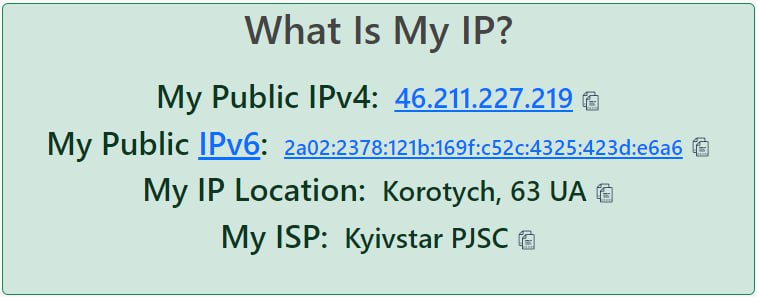
\includegraphics[width=0.90\textwidth]{myip.jpg}
    \caption{Публічний ІР}
\end{figure}


\begin{figure}[H]
    \centering
    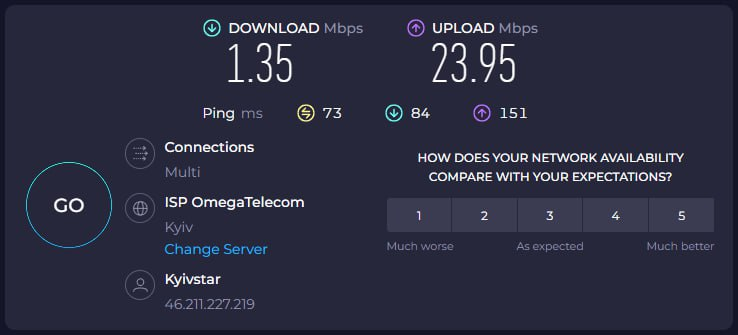
\includegraphics[width=0.90\textwidth]{speedtest.jpg}
    \caption{Швидкість мобільного інтернету в лекційній авдиторії}
\end{figure}

\begin{figure}[H]
    \centering
    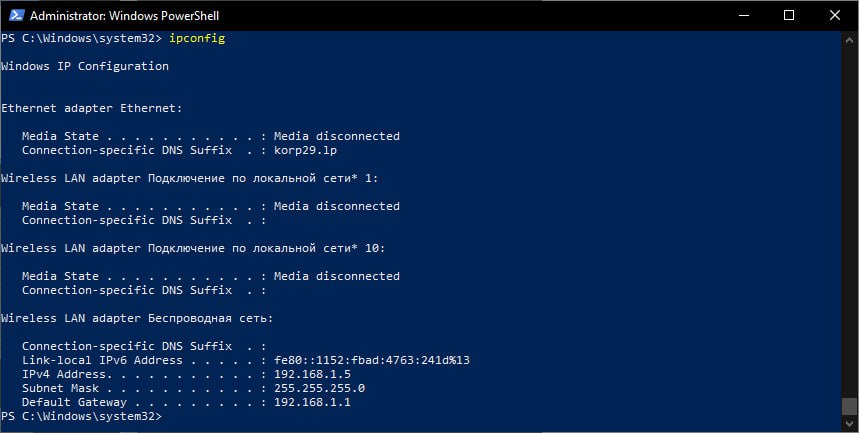
\includegraphics[width=0.90\textwidth]{ipconfig.jpg}
    \caption{}
\end{figure}

\begin{figure}[H]
    \centering
    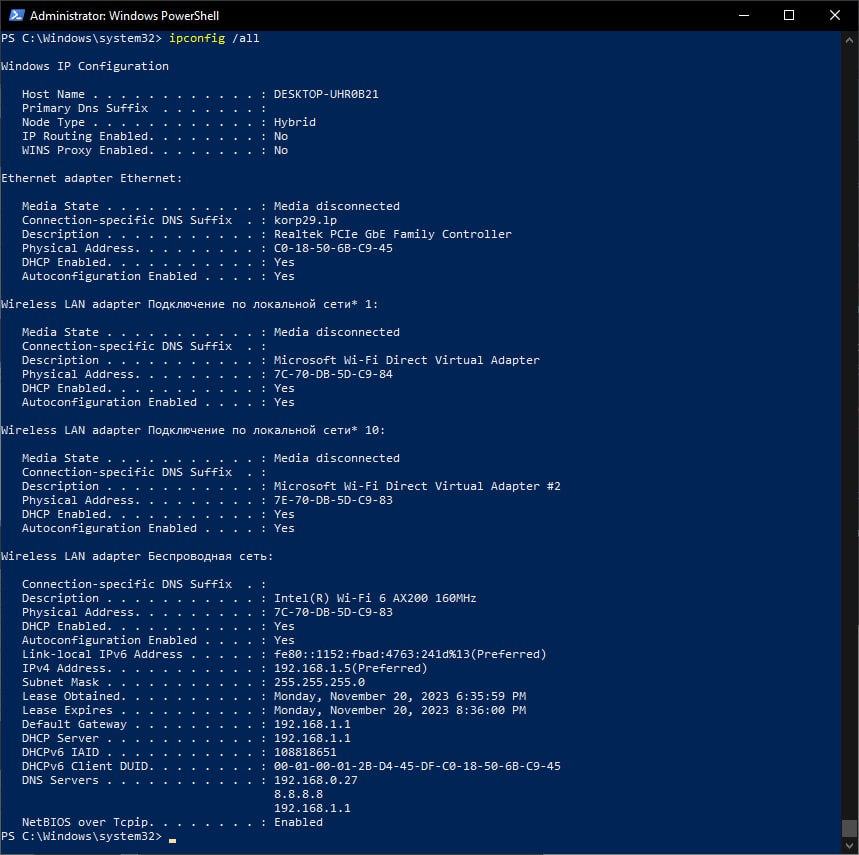
\includegraphics[width=0.90\textwidth]{all.jpg}
    \caption{}
\end{figure}

\begin{figure}[H]
    \centering
    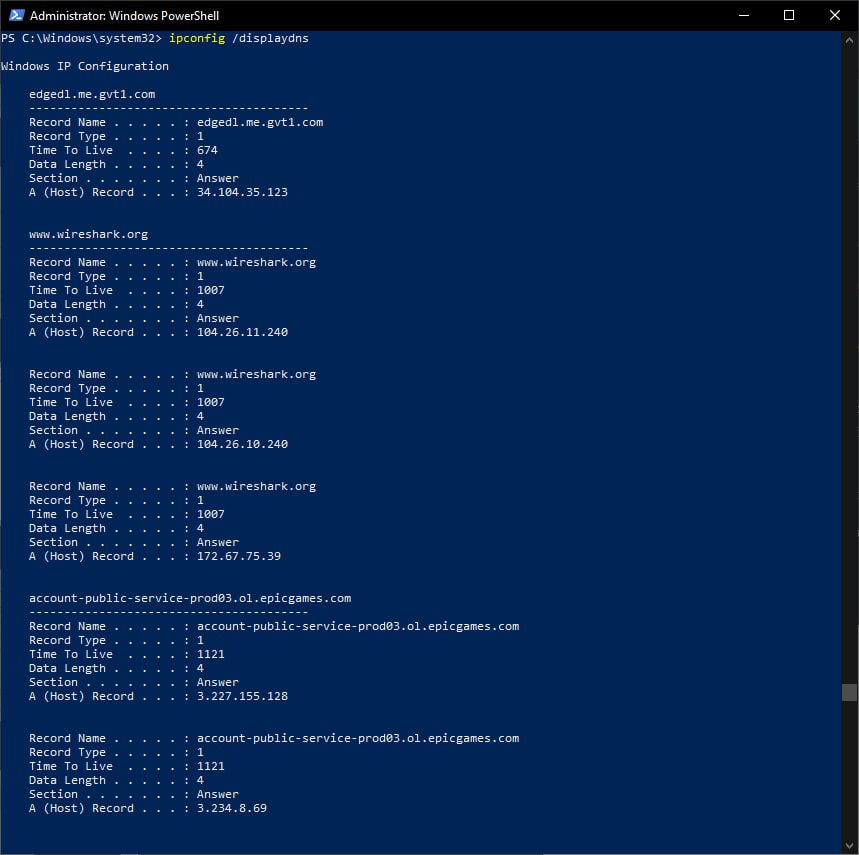
\includegraphics[width=0.90\textwidth]{displaydns.jpg}
    \caption{}
\end{figure}
\begin{figure}[H]
    \centering
    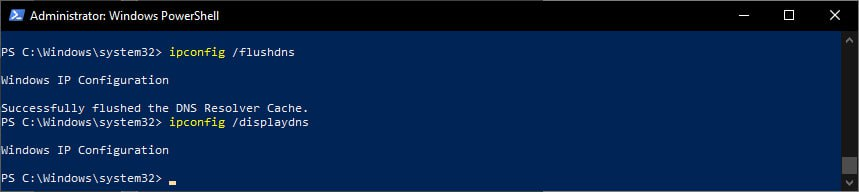
\includegraphics[width=0.90\textwidth]{flushdns.jpg}
    \caption{}
\end{figure}
\begin{figure}[H]
    \centering
    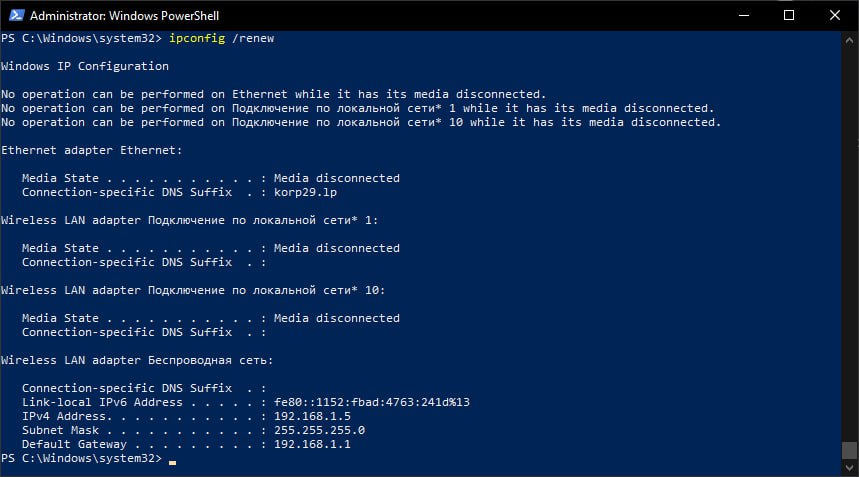
\includegraphics[width=0.90\textwidth]{renew.jpg}
    \caption{}
\end{figure}
\begin{figure}[H]
    \centering
    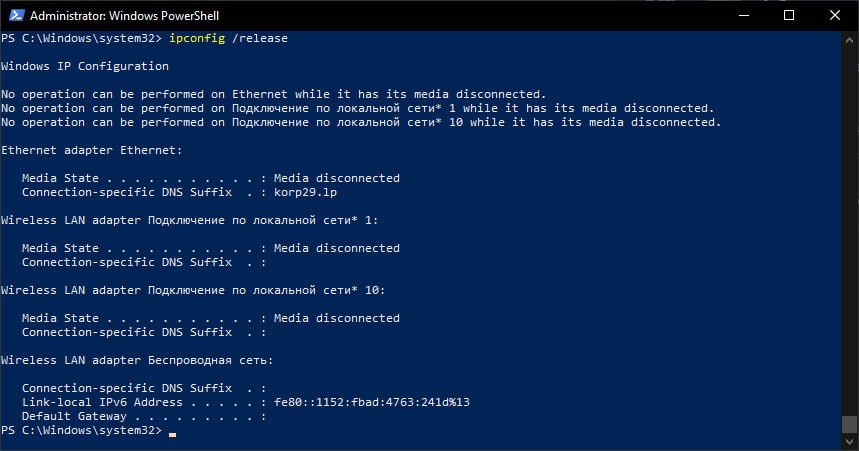
\includegraphics[width=0.90\textwidth]{release.jpg}
    \caption{}
\end{figure}
\begin{figure}[H]
    \centering
    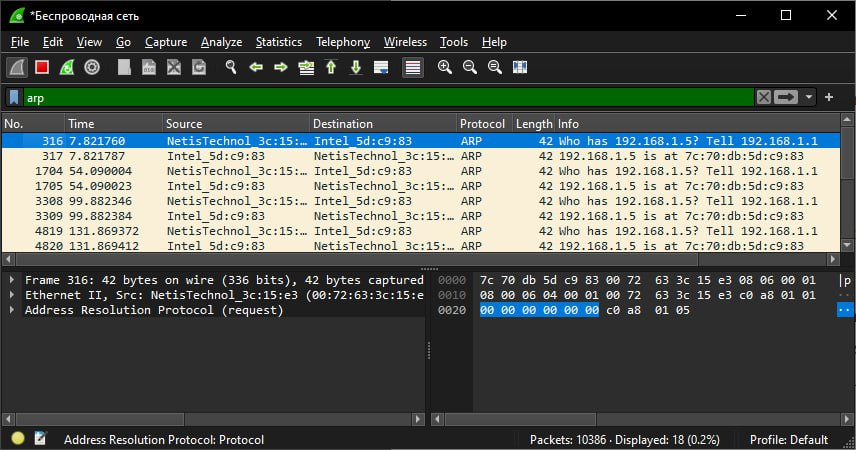
\includegraphics[width=0.90\textwidth]{arp.jpg}
    \caption{}
\end{figure}
\begin{figure}[H]
    \centering
    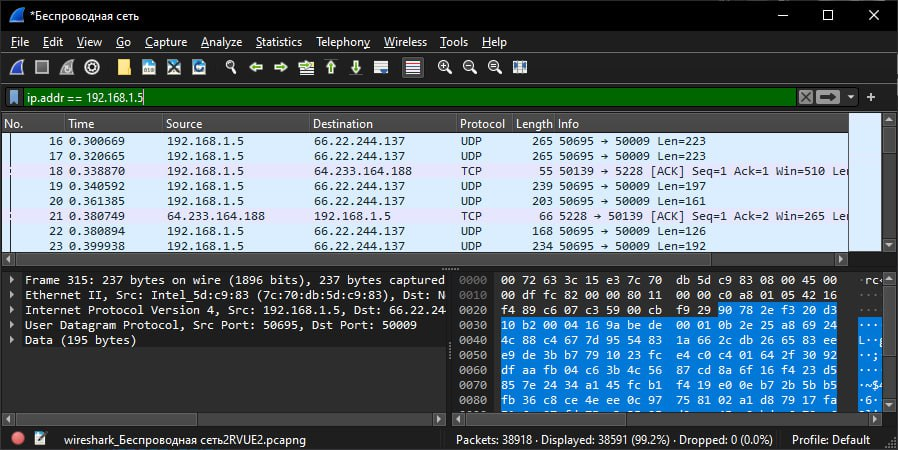
\includegraphics[width=0.90\textwidth]{ip_search.jpg}
    \caption{}
\end{figure}
\vspace{12pt}

\subsection*{Висновок} 
Я навчився як можна дізнатись свою публічну і локальну ІР-адресу,
що таке ARP протокол і як подивитись ARP-таблицю, як користуватись
Wireshark і фільтрувати пакети за допомогою нього.
\end{document}